\section{Antennen}
\subsection{Herz'scher Dipol (HDp)}
\subsubsection{Allgemein}
$ r $: Antennen\textbf{abstand}
{\footnotesize\begin{empheq}[box=\fbox]{align*}
		{\vec{\underline{H}}} & =-\frac{I_0\Delta l'\beta^2}{4\pi}e^{-j\beta r}\cdot\sin\vartheta\left(\frac{1}{j\beta r}+\frac{1}{(j\beta r)^2}\right)\vec{e}_\varphi                                 \\
		{\vec{\underline{E}}} & = -\frac{Z_F I_0\Delta l'\beta^2}{2\pi}e^{-j\beta r}\cdot\cos\vartheta\left(\frac{1}{(j\beta r)^2}+\frac{1}{(j\beta r)^3}\right)\vec{e}_r                           \\
		& -\frac{Z_F I_0\Delta l'\beta^2}{4\pi}e^{-j\beta r}\cdot\sin\vartheta\left(\frac{1}{(j\beta r)}+\frac{1}{(j\beta r)^2}+\frac{1}{(j\beta r)^3}\right)\vec{e}_\vartheta
	\end{empheq}}

Im Zeitbereich:
{\footnotesize\begin{align*}
	E_r (t)         & = \frac{Z_F I_0 l}{2\pi r^3 \beta}\cos \vartheta \left[ \sin (\omega t- \beta r) + \beta r \cos (\omega t - \beta r) \right]                                        \\
	E_\vartheta (t) & = \frac{Z_F I_0 l}{4\pi r^3 \beta}\sin \vartheta \left[ \sin (\omega t- \beta r) + \beta r \cos (\omega t - \beta r) - (\beta r)^2 \sin(\omega t - \beta r) \right] \\
	H_\varphi (t)   & = \frac{I_0 l}{4\pi r^2 }\sin \vartheta \left[ \cos (\omega t- \beta r) + \beta r \sin (\omega t - \beta r) \right]
\end{align*}}

\subsubsection[Nahfeld]{Nahfeld (Fresnel-Zone)} $\frac{\lambda}{2\pi R}\gg 1$ oder $\beta R \ll 1$ oder $ r \ll \lambda $ \qquad  $ \approx $  Faktor 10\\
Überwiegend \textbf{Blindleistungsfeld}, da $\vec{E}$ zu $\vec{H}$ $90^\circ$
phasenverschoben. Lösung entspricht dem quasistatischem Dipolfeld.
$\rightarrow$ \textbf{keine} Wellenausbreitung!
\begin{empheq}[box=\fbox]{align*}
	\vec{\underline{H}} & \approx \frac{I_0 \Delta l'}{4\pi r^2}\cdot\sin\vartheta\cdot\vec{e}_\varphi                                            \\
	\vec{\underline{E}} & \approx \frac{I_0 \Delta l'}{2\pi j \omega\varepsilon r^3}\cos\vartheta\cdot\vec{e}_r
	+       \frac{I_0 \Delta l'}{4\pi j \omega\varepsilon r^3}\sin\vartheta\cdot\vec{e}_\vartheta
\end{empheq}

\subsubsection[Fernfeld]{Fernfeld (Fraunhofer-Zone)}

$\frac{\lambda}{2\pi R}\ll 1$ oder $\beta R\gg 1$ oder $ r \gg \lambda $ \qquad
$\approx$ Faktor 10\\

Überwiegend \textbf{Wirkleistungsfeld}, $\vec{S}$ in Richtung $\vec{e}_r$

$ \rightarrow $ Kugelwelle, $\vec{E}$ und $\vec{H}$ in Phase, fallen mit $
	\frac{1}{r} $ ab.

\vspace{1ex}
\begin{empheq}[box=\fbox] {align*}
	\vec{\underline{H}} & \approx  j\frac{\beta I_0 \Delta l'}{4\pi r}\cdot e^{-j\beta r}\cdot\sin\vartheta\cdot\vec{e}_\varphi                           \\
	\vec{\underline{E}} & \approx  j\frac{\beta Z_F I_0 \Delta l'}{4\pi r}\cdot e^{-j\beta r}\cdot\sin\vartheta\cdot \vec{e}_\vartheta
\end{empheq}

\subsubsection{Abgestrahlte Leistung im Fernfeld HDp}
\begin{align*}
	P_\texttt{rad} = P_s & = \frac{Z_{F0} {I_0}^2 \beta^2 (\Delta l')^2}{12\pi}
	= \frac{I_0^2 Z_F\pi}{3}\cdot \dfrac{\Delta l'^2}{\lambda^2}                                               \\
	                     & = 40\pi^2\Omega\cdot\left(\frac{I_0\Delta l'}{\lambda}\right)^2                     \\
	\vec{S}_{av}         & = \frac{Z_FI_0^2\beta^2(\Delta l')^2}{32\pi^2r^2}\cdot\sin^2\vartheta\cdot\vec{e}_r \\
	                     & = \frac{1}{2}\Re\left\{\vec{E}\times\vec{H}^*\right\}
\end{align*}

\subsubsection{Strahlungswiderstand HDp}
\begin{align*}
	R_s & = \frac{2}{3}\pi Z_F\left(\frac{\Delta l'}{\lambda}\right)^2
	= 80\pi^2\Omega\left(\frac{\Delta l'}{\lambda}\right)^2
\end{align*}

\subsubsection{Verlustwiderstand HDp}
\begin{align*}
	R_{v} & = \frac{l}{\sigma\cdot A_\delta} \qquad \text{siehe Skin-Effekt}
\end{align*}

\subsection{Magnetischer Dipol}
Dipolmoment: \boxed{\vec{m} = \vec{I}\pi\vec{a}^2\vec{e}_z}
\boxed{m = I\cdot A}
\begin{center}
	\input{Figures/Antennen_Magnetischer_Dipol.tex}
\end{center}

{\footnotesize\begin{empheq}[box=\fbox]{align*}
	{\vec{\underline{H}}}   & = -\frac{j\omega\mu\beta^2m}{2\pi Z_{F0}}e^{-j\beta r}\cdot\cos\vartheta\left(\frac{1}{(j\beta r)^2}+\frac{1}{(j\beta r)^3}\right)\vec{e}_r                             \\
	&	 -\frac{j\omega\mu\beta^2m}{4\pi Z_{F0}}e^{-j\beta r}\cdot\sin\vartheta\left(\frac{1}{(j\beta r)}+\frac{1}{(j\beta r)^2}+\frac{1}{(j\beta r)^3}\right)\vec{e}_\vartheta   \\
	{\vec{\underline{E}}}   & =  \frac{j\omega\mu\beta^2m}{4\pi}e^{-j\beta r}\sin\vartheta\left(\frac{1}{j\beta r}+\frac{1}{(j\beta r)^2}\right)\vec{e}_\varphi
\end{empheq}}

mag. Vektorpotenzial $ \vec{A} $:
\begin{flalign*}
	\vec{A} & = \frac{\mu m}{4\pi r^2}(1+j\beta r) e^{-j\beta r}\sin\vartheta\cdot\vec{e}_\varphi
\end{flalign*}

$ P_{rad} $: elek. Dipol der Länge l $\widehat{=}$ mag. Dipol der Fläche A
\begin{align*}
	\Delta l & = \beta \cdot A_{\texttt{Kreis}} = \beta \cdot \pi\ a^2 & \frac{m}{v_p}=p &
\end{align*}

\subsubsection{Fernfeld}
\begin{empheq}[box=\fbox]{align*}
	E & \approx -\frac{\beta m\omega\mu}{4\pi r}e^{-j\beta r}\sin\vartheta\cdot\vec{e}_\varphi \\
	H & \approx -\frac{\beta m\omega\mu}{4\pi r Z_{F0}}e^{-j\beta r}\sin\vartheta\cdot\vec{e}_\vartheta
\end{empheq}

\subsubsection{Abgestrahlte Leistung im Fernfeld}
\begin{align*}
	P_\texttt{rad} = P_s & = \frac{Z_F\beta^4m^2}{12\pi}
	= \frac{m^2\mu\omega^4}{12\pi v_p^3}                                                        \\
	S_{av}               & = \frac{Z_F\beta^4m^2}{32\pi^2r^2}\cdot\sin^2\vartheta\cdot\vec{e}_r \\
	                     & = \frac{1}{2} Re\left\{\vec{E}\times\vec{H}^*\right\}
\end{align*}

\subsubsection{Nahfeld}
\begin{empheq}[box=\fbox]{align*}
	E & \approx -\frac{jm\omega\mu}{4\pi r^2}\sin\vartheta\cdot\vec{e}\varphi \\
	H & \approx \frac{m}{4\pi r^3}(2\cos\vartheta\cdot\vec{e}_r+\sin\vartheta\cdot\vec{e}_\vartheta)
\end{empheq}

\newpage
\subsection{Lineare Antenne}
Stromverteilung auf linearen Antennen \textbf{nicht} konstant:
\begin{align*}
	I(z') & = I_0\cdot\sin\left[\beta\left(\frac{l}{2}-|z'|\right)\right]
\end{align*}

\subsubsection{Dipolantenne allgemein}
$ l $: Antennen\textbf{länge} \qquad $ r $: Antennen\textbf{abstand}
\begin{align*}
	\vec{\underline{H}} & = j\frac{I_0}{2\pi r}\cdot e^{-j\beta r}\cdot\frac{\cos\left[\left(\frac{\beta l}{2}\right)\cos\vartheta\right]-\cos\left(\frac{\beta l}{2}\right)}{\sin\vartheta}\cdot\vec{e}_\varphi \\
	\vec{\underline{E}} & = H\cdot Z_{F0}\cdot\vec{e}_\vartheta                                                                                                                                                  \\
	I_0                 & = \sqrt{\frac{2\cdot P_{s}}{R_{s}}} \qquad R_{s} \rightarrow \text{siehe Antennentabelle Kap. \ref{sec:Antennentabelle}}
\end{align*}

\textbf{Halbwellen}dipol: $ l=\frac{\lambda}{2} \qquad
	\underline{Z}_{s}=(\overbrace{73,13}^{R_s}+j\overbrace{42,54}^{X_s})\Omega$

\textbf{Ganzwellen}dipol: $ l=\lambda \qquad \underline{Z}_{s}=(199,09+j125,41)\Omega$

\subsubsection{Eingangs-/Fußpunktimpedanz}
Bei leerlaufender Leitung entstehen in Längsrichtung stehende Wellen. Um max.
Wirkleistung zu übertragen, muss die Eingangs-/Fußpunktimpedanz $ Z_A $
\textbf{reell} bzw. die Leitung in Resonanz sein.

\begin{equation*}
	P_{max} \rightarrow n \cdot \frac{\lambda}{4}
\end{equation*}

\begin{align*}
	\underline{Z}_A & =\underline{Z}_s\frac{|I_0|^2}{|I_0(z'=0)|^2} = \frac{\underline{Z}_s}{\sin^2\left[ \beta \frac{l}{2} \right] }
\end{align*}

Strom am Fußpunkt:
\begin{align*}
	I(z'=0) & = I_0\cdot\sin\left[\beta\left(\frac{l}{2}\right)\right]
\end{align*}

Komplexe Strahlungsleistung:
\begin{align*}
	P_s +jQ_s = \underline{Z}_s\cdot \frac{|I_0|^2}{2} = \underline{Z}_A \cdot \frac{|I_0(z'=0)|^2}{2}
\end{align*}

\subsubsection{Strahlungsdichte}
\begin{align*}
	\vec{S}_{av} & = \frac{Z_FI_0^2}{8\pi^2 r^2}\left(\frac{\cos\left(\frac{\beta l }{2}\cos\vartheta\right)-\cos\left(\frac{\beta l}{2}\right)}{\sin\vartheta}\right)^2\cdot\vec{e}_r \\
	S_{av}       & = S_{iso} \cdot D_{max} \cdot C^2(\vartheta, \varphi)                                                                                                               \\
	S            & = S_{iso} \cdot G \cdot \eta
\end{align*}

\subsubsection{abgestrahlte Wirkleistung}
\begin{align*}
	P_{s} & = \int_A S_{av}\cdot d\vec{a}                                                                                                                                                           \\
	      & = \int^{2\pi}_{\varphi = 0}\int^{\pi}_{\vartheta = 0} S_{av}\cdot r^2 \sin\vartheta \, d\vartheta \, d\varphi                                                                           \\
	P_{s} & = \frac{Z_{F}I_0^2}{4\pi}\cdot\int^{\pi}_{\vartheta=0}\frac{\left(\cos\left(\frac{\beta l}{2}\cos\vartheta\right)-\cos\left(\frac{\beta l}{2}\right)\right)^2}{\sin\vartheta}d\vartheta \\
	      & = \frac{Z_{F}I_0^2}{4\pi}\cdot x
\end{align*}

Numerische Lösung des Integrals ergibt Faktor $ x $:\\
bei \textbf{Halbwellen}dipol: $ x=1,2188 $\\
bei \textbf{Ganzwellen}dipol: $ x=3,3181$


\newcolumn
\subsection{Antennenkenngrößen}
\input{Figures/Antennen_Antennenkenngroessen_circuit.tex}

$ X_A $ wird kompensiert $ \rightarrow $ max. Wirkleistungsübertragung

\subsubsection{Abgestrahlte Leistung}
\begin{align*}
	P_s = P_{rad} & = \frac{1}{2}\cdot I_A^2 \cdot R_s
\end{align*}

\subsubsection{Verlustleistung}
\begin{align*}
	P_V & = \frac{1}{2}\cdot I_A^2\cdot R_V
\end{align*}

\subsubsection{Wirkungsgrad}
wenn $ R_V $ vorhanden $\rightarrow$ wirkt sich auf $ G $ aus!
\begin{align*}
	\eta & = \frac{P_s}{P_s + P_V} = \frac{R_s}{R_s + R_V}
\end{align*}

\subsubsection{Gewinn/Gain}
Verlustlose Antenne, wenn $ \eta = 1 $
\begin{align*}
	G & = \eta \cdot D & [1]\\
    g &= 10 \cdot log(G) & [\si{dB}]
\end{align*}

\subsubsection{Richtcharakteristik (Feldstärke)}
$C_{i} \ent$ isotroper Kugelstrahler als Bezugsgröße in Hauptabstrahlrichtung
\begin{align*}
	C_{i}(\vartheta, \varphi) & = \frac{E(\vartheta, \varphi)}{E_{i}}=\frac{H(\vartheta, \varphi)}{H_{i}}                                               & C_{i}>1                             \\
	C(\vartheta, \varphi)     & = \frac{E(\vartheta, \varphi)}{E_{\max}}=\frac{H(\vartheta, \varphi)}{H_{\max}} = \frac{U(\vartheta,\varphi)}{U_{\max}} & 0 \leq C(\vartheta, \varphi) \leq 1 \\
	C(\vartheta, \varphi)     & = \left|\frac{\cos\left(\frac{\beta L}{2}\cos\vartheta\right)-\cos\left(\frac{\beta L}{2}\right)}{\sin\vartheta}\right| \\
	                          & \text{\textbf{Halbwellen}dipol}\quad l=\frac{\lambda}{2} \\
	C(\vartheta, \varphi)     & = \frac{\cos\left(\frac{\pi}{2}\cos\vartheta\right)}{\sin\vartheta}    \\
	                          & \text{\textbf{Ganzwellen}dipol}\quad l=\lambda           \\ 
    C(\vartheta, \varphi)     &= \frac{\cos\left(\pi\cos\vartheta\right)+1}{2\sin\vartheta}
\end{align*}

\subsubsection{Richtfunktion/-faktor (Leistungsgröße)} 
\begin{align*}
	D_{\texttt{eff}}(\vartheta, \varphi) & = \frac{S(\vartheta, \varphi)}{S_{i}} = C^\mathbf{2}_i(\vartheta, \varphi) = D_{\texttt{max}} \cdot C^\mathbf{2}(\vartheta, \varphi) & \\
	D_{max}                              & = \max \{D(\vartheta, \varphi)\} = \frac{S_{\max}}{S_{i}}                                                                            &
\end{align*}

\vspace{-0.5cm}
\begin{align*}
	                                                                                          & \text{\textbf{Halbwellen}dipol}\quad l=\frac{\lambda}{2} \\
	                                                                                          & D_{\texttt{eff}}(\vartheta, \varphi) = 1,64 \cdot
	\left(\frac{\cos\left(\frac{\pi}{2}\cos\vartheta\right)}{\sin\vartheta}\right)^\mathbf{2} &                                                          \\
	                                                                                          & \text{\textbf{Ganzwellen}dipol}\quad l=\lambda           \\ &D_{\texttt{eff}}(\vartheta, \varphi) = 2,41 \cdot
	\left(\frac{\cos\left(\pi\cos\vartheta\right)+1}{2\sin\vartheta}\right)^\mathbf{2}        &
\end{align*}

\paragraph{Abstrahlwinkel}
(meist $\vartheta$)\\
\begin{tikzpicture}
    \draw[-] (-2,0) node[left] {$270^{\circ}/\dfrac{3\pi}{2}$}
        -- (2,0) node[right] {$90^{\circ}/\dfrac{\pi}{2}$};
    \draw node[right,text width=1.5cm] () at (3,0) {Meist Hauptabstrahlrichtung};
    \draw[-] (0,-2) node[below] {$180^{\circ}/\pi$}
        -- (0,2) node[above] {$0^{\circ}/0\pi/2\pi$};
    \draw[dotted] (0,0) -- (1,1.732) node[above right, fill=black!5] {$30^{\circ}/\dfrac{\pi}{6}$};
    \draw[dotted] (0,0) -- (2,1.154) node[right, fill=black!5] {$60^{\circ}/\dfrac{\pi}{3}$};
    \draw[dotted] (0,0) -- (2,-1.154) node[right, fill=black!5] {$120^{\circ}/\dfrac{2\pi}{3}$};
    \draw[dotted] (0,0) -- (1,-1.732) node[below right, fill=black!5] {$150^{\circ}/\dfrac{5\pi}{6}$};
\end{tikzpicture}


\subsection{Senden und Empfangen}
Bei Anpassung: $R_e = R_s \rightarrow$ max. Wirkleistung wird übertragen!
\begin{center}
    \resizebox{0.75\columnwidth}{!}{
        \begin{circuitikz}
            %Schaltbild
            \draw(0,0) node[below right]{$U_0=l_{\texttt{eff}}\cdot E$}
            to[V,v=$U_0 $](0,2)                               %Spannungsquelle
            to[R=$R_{S}$](2,2)                                   %Strahlungswiderstand
            to[short](4 ,2)
            to[R= $R_{E}$](4,0)
            to[short](0,0);
            \draw(3,2) node[below]{$l$}
            to[open,o-o](3,0) node[above]{$l'$};

        \end{circuitikz}
    }
\end{center}


$ R_s $: Strahlungswiderstand \quad $ s $: Sender \qquad $ e $: Empfänger\\
$ r $: \textbf{Abstand} von der Antenne

\begin{align*}
	P_e & = \frac{1}{2}\cdot R_s \cdot I^2 = \frac{U_0^2}{8R_{s}} \qquad S_s = \frac{1}{2}\, H_0^2 \, Z_{F0} = \frac{1}{2} \, \frac{E_0^2}{Z_{F0}} \\
	    & = \frac{E_0^2\cdot l^2_{\mathtt{eff}}}{8R_{s}}
\end{align*}

\subsubsection{Wirksame/Effektive Antennenfläche}
\begin{align*}
	A_\texttt{eff} & = \frac{P_e}{S_s} = \frac{U_0^2}{8R_{s}}\frac{2Z_{F0}}{E_0^2}                  &
	A_{\mathtt{eff,n}}\Big|_{\mathtt{max}} & = \frac{\lambda^2}{4\pi}\cdot G_n = \dfrac{Z_{F0}}{4 R_S} \cdot l_\texttt{eff}^2 &
\end{align*}

Beim Hertzschen Dipol:
\begin{align*}
	A_\texttt{eff} & =  \frac{\lambda^2}{4\pi}\cdot\frac{3}{2}\sin^2\vartheta &
\end{align*}

\subsubsection{Friis-Übertragungsgleichung}
\begin{align*}
	 & S_{iso} = \frac{P_s}{4\pi r^2}                                                       & S_s = S_{iso} \cdot D_s                                                  \\
	 & S_n=\frac{P_s}{4\pi r^2}\cdot G_n = \frac{P_s}{4\pi r^2}\cdot D_n(\vartheta, \varphi)\cdot \eta_n                                                                                                              
\end{align*}
\begin{align*}
	P_e                                     & = S_s \cdot A_{\mathtt{eff,e}} = S_s\cdot \frac{\lambda^2}{4\pi}\cdot D_e(\vartheta, \varphi)\cdot \eta_e                                                \\
	\frac{P_{e}}{P_{s}}                     & = A_{\texttt{eff},e}\cdot A_{\texttt{eff},s}\cdot\frac{1}{\lambda^2r^2}                                                    \\
	                                        & = D_e(\vartheta, \varphi)\cdot\eta_{e}\cdot D_s(\vartheta, \varphi)\cdot\eta_{s}\cdot\left(\frac{\lambda}{4\pi r}\right)^2 \\
	\frac{P_{e}}{P_{s}}\Big|_{\mathtt{max}} & = G_{s}\cdot G_{e}\cdot \left(\frac{\lambda}{4\pi r}\right)^2
\end{align*}

Reziprozität: Sende- und Empfangscharakteristik sind identisch!

\subsubsection{Freiraumdämpfung (Leistung)}
d: Abstand zur Antenne
\begin{align*}
	F = \dfrac{P_{s}}{P_{e}} \cdot \left(\dfrac{4 \pi d}{\lambda}\right)^2                             & \qquad [1]       \\
	a_{0} = 20 \log \left(\frac{4 \pi d}{\lambda}\right) =20 \log \left(\frac{4 \pi d f}{c_{0}}\right) & \qquad [\si{dB}]
\end{align*}

\subsubsection{Leistungspegel/Freiraumpegel}
\begin{align*}
	L     & = 10 \lg \left(\frac{P}{1 \si{mW}}\right) \qquad [\si{dBm}] \\
	L_{e} & = L_{s}+g_{s}+g_{s}-a_{0} \qquad [\si{dB}]
\end{align*}

\subsection{Bezugsantennen}
\[
	\boxed{g = 10 \cdot log(G) \si{dB}}
\]

mit $P_0$ : Eingangsleistung der Antenne

\begin{description}
	\item \textbf{\underline{G$\rightarrow$Bezugsantenne:}}

	      Elementardipol  zu Kugelstrahler \[D = 1,50 \rightarrow g = 1,76\si{dBi}\]
	      Halbwellendipol zu Kugelstrahler \[D = 1,64 \rightarrow g = 2,15\si{dBi}\]

	\item \textbf{\underline{EIRP}: Eqivalent \underline{Isoropic} Radiated Power}
	      \[
		      \text{EIRP} = P_0 \cdot G_i \qquad [\si{dBi}]
	      \]
          \si{dBi} Bezugsantenne isotroper Kugelstrahler

	\item \textbf{\underline{ERP}: Effective Radiated Power (verlustloser Halbwellendipol)}
	      \[
		      \text{ERP} = P_0 \cdot G_d \qquad [\si{dBd}]
	      \]
          \si{dBd} Bezugsantenne Halbwellendipol
          \[
            0 \si{dBd} = 2,15 \si{dBi}
          \]
          \[
            y \si{dBd} + 2,15 \si{dBi} = x \si{dBi}
          \]
\end{description} 

\subsection{Monopolantenne}
Verhält sich wie ein Dipol, der nur in die obere Hälfte abstrahlt.
\begin{align*}
    R_S &= \dfrac{1}{2} \cdot R_{S,DP}\\
    D &= 2 \cdot D_{DP}
\end{align*}

Geometrisch zu kurze Antennen können durch breiteren Drahtdurchmesser,
Fußpunktinduktivität oder Dachkapazität elektrisch verlängert werden.